\section{Three questions, three checks}
\label{sec:checks}

In this section we define the three checks and prove what each one delivers.
We state the definitions in words here. Appendix~\ref{app:models} gives them in
full for each model, and Appendix~\ref{app:index} names the Lean declarations.

\subsection{Realization on the target}
\label{sec:realization}

We assemble a realization on the target from local pieces, one for each
condition. Each piece reads some of the target's cells: tables of transition
weights, positions, records and so on. It must be accepted by its own
condition. We ask when accepted pieces fit together into one assignment of values to all
the cells.

\begin{definition}[Cover with running intersection]
% claim: TTH-01
\label{def:cover}
A \emph{cover} is a family of pieces, each with a scope (the cells it reads),
such that every cell lies in some scope, together with an adjacency relation
on pieces. It has the \emph{running-intersection} property if any two pieces
whose scopes contain a cell $c$ are joined by a path of adjacent pieces whose
scopes all contain $c$. Local assignments are \emph{compatible along edges} if
adjacent pieces assign the same value to every cell they share.
\end{definition}

\begin{theorem}[Gluing]
% claim: TTH-01
\label{thm:gluing}
Let a rooted cover have the running-intersection property, and let local
assignments be compatible along edges. Then there is a global assignment whose
restriction to each piece's scope is that piece's local assignment.
\end{theorem}

We prove it by propagating equality along the paths that running intersection
provides. The acceptance of the global assignment is not a conclusion of the
theorem. It comes from each piece's own acceptance, which the realization
check records separately. The same idea is standard for acyclic database
schemes, where pairwise consistency gives global consistency exactly when the
scheme is acyclic \citep[Theorem~3.4]{BeeriEtAl1983}.

On the models of Section~\ref{sec:continuation}, a realization on the target is
built in stages. Typed maps carry each condition's cells from the source to
the target. Each mapped piece is then accepted, independently, by its own
condition on the target, and a compatible cover on the target, also checked
independently, glues the pieces. The assembly uses no premise about lineage or autonomy. Realization,
in other words, can be established without knowing how the target came to be.

We cannot drop running intersection.

\begin{proposition}[Agreement between neighbours is not enough]
% claim: TTN-08
\label{prop:cycle}
On the target of the two-copy model there are eight local assignments, one for
each condition, each accepted and gated by its own condition, such that
adjacent pieces agree on every cell they share, where adjacency forms a cycle
through the eight conditions. Yet no global assignment restricts to all eight.
\end{proposition}

\begin{figure}[tbp]
\centering
% F3: running-intersection schematic and the actual cycle's conflicting cell.
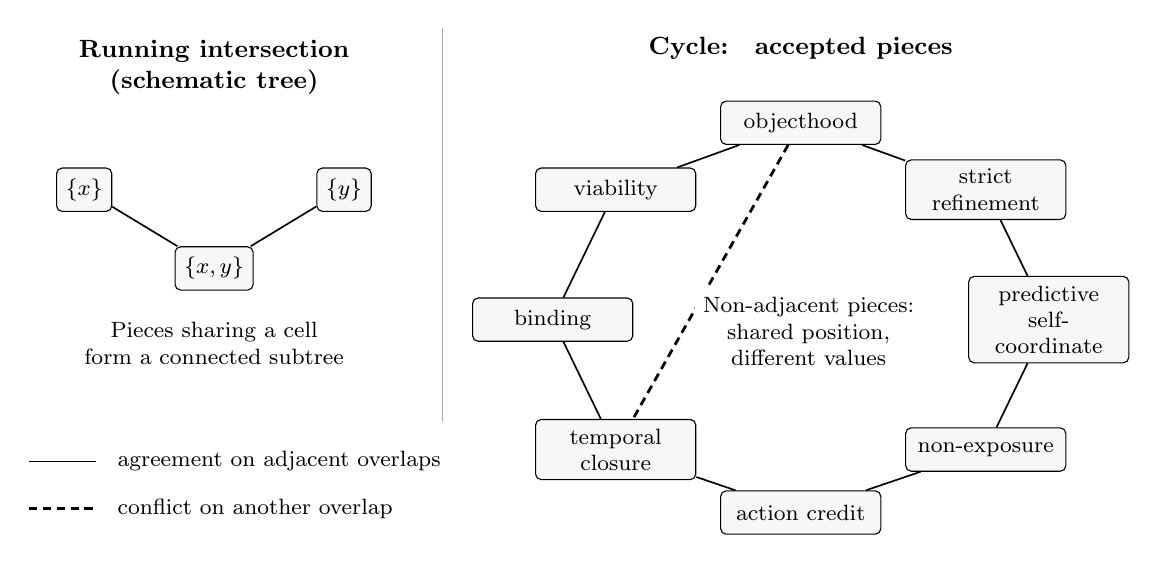
\begin{tikzpicture}[x=1cm,y=1cm,font=\footnotesize,
 piece/.style={draw,rounded corners=2pt,fill=black!3,align=center,minimum height=.55cm},
 adjacent/.style={semithick},conflict/.style={densely dashed,line width=1pt}]
\node[font=\small\bfseries,align=center] at (2.65,3.45) {Running intersection\\(schematic tree)};
\node[piece] (a) at (1,1.9) {$\{x\}$};
\node[piece] (b) at (2.65,.9) {$\{x,y\}$};
\node[piece] (c) at (4.3,1.9) {$\{y\}$};
\draw[adjacent] (a)--(b)--(c);
\node[align=center] at (2.65,-.05) {Pieces sharing a cell\\form a connected subtree};
\draw[black!35] (5.55,-1.05)--(5.55,3.95);
\node[font=\small\bfseries] at (10.1,3.7) {Cycle: \snapPosZeroFourStagedClauseCount{} accepted pieces};
\node[piece,text width=1.8cm] (obj) at (10.1,2.75) {objecthood};
\node[piece,text width=1.8cm] (refine) at (12.45,1.9) {strict\\refinement};
\node[piece,text width=1.8cm] (predict) at (13.25,.25) {predictive\\self-coordinate};
\node[piece,text width=1.8cm] (privacy) at (12.45,-1.4) {non-exposure};
\node[piece,text width=1.8cm] (credit) at (10.1,-2.2) {action credit};
\node[piece,text width=1.8cm] (time) at (7.75,-1.4) {temporal closure};
\node[piece,text width=1.8cm] (binding) at (6.95,.25) {binding};
\node[piece,text width=1.8cm] (viable) at (7.75,1.9) {viability};
\draw[adjacent] (obj)--(refine)--(predict)--(privacy)--(credit)--(time)--(binding)--(viable)--(obj);
\draw[conflict] (obj)--(time);
\node[align=center,fill=white,inner sep=3pt] at (10.2,.1) {Non-adjacent pieces:\\shared position,\\different values};
\draw[adjacent] (.3,-1.55)--(1.15,-1.55);
\node[anchor=west] at (1.3,-1.55) {agreement on adjacent overlaps};
\draw[conflict] (.3,-2.15)--(1.15,-2.15);
\node[anchor=west] at (1.3,-2.15) {conflict on another overlap};
\end{tikzpicture}

\caption{Gluing and its failure. On the left, when the pieces that share a cell form a connected subtree, agreement on adjacent overlaps glues. On the right, eight accepted pieces, one per condition, agree on every adjacent overlap, but two non-adjacent pieces read the same position table with different values, so no global assignment exists. The cycle is incidental, and the failure is one of running intersection.}
\label{fig:gluing}
\end{figure}

The obstruction is local and simple. Two pieces that are not adjacent both read
the table of positions and disagree on one entry, and neither neighbour of one
of them reads that table. So the scope of that table is not connected, and
running intersection fails. The cycle plays no role: a path of pieces with the
same scopes would fail in the same way. What matters is that checking
agreement only between neighbours misses a disagreement that running
intersection would have exposed.

Public observations also lose information that the checks use. This is the
formal version of the public shadow of Section~\ref{sec:copy}.

\begin{proposition}[Public shadow]
% claim: TTN-02
\label{prop:shadow}
On the target of the two-copy model there are two states that give identical
readings on every channel of the fixed public interface, while their
predictive readouts differ.
\end{proposition}

The interface here is the fixed list of public channels of the two-copy model.
The proposition says nothing about every possible observation.

\subsection{Lineage}
\label{sec:lineage}

We check lineage one handoff at a time. A \emph{handoff} is a finite
sequence of stages from a source system to a distinct target system. Each
stage records which systems are live in it and a frontier of the eight
temporal fields of Section~\ref{sec:setting}.

\begin{definition}[Strict handoff]
% claim: TTH-04
\label{def:handoff}
A handoff is \emph{strict} if it passes every check of the formal atomic
gate, expanded in Appendix~\ref{app:checks}. In summary, the gate
requires the following.
\begin{itemize}
\item Source and target are distinct, and there are at least three stages.
\item Only the source is live at entry and only the target at exit.
\item Some stage has both live: this is the overlap.
\item Every stage is realized, so there is no gap.
\item Each step from one stage to the next increases order, tick, progress
and records by a strictly positive amount, extends the route memory, and keeps
an owner among the live systems.
\item Events have unique identifiers, valid stages and owners, and their
dependencies point forward.
\item Every stage has a nonempty maintenance state.
\item An intervention check shows that both systems' contributions are needed,
and an audit check holds.
\item The route is recorded as route-indexed.
\end{itemize}
A \emph{strict chain} is a nonempty list of strict handoffs in which each
handoff ends exactly where the next begins: the same intermediate system and
the same boundary stage, including its whole frontier. Its first source and
last target must differ.
\end{definition}

\begin{proposition}[Strict chains]
% claim: TTH-04
\label{prop:chain}
Every strict chain admits an inductive derivation from its handoffs. Every
stage of the concatenated chain is realized, and every step strictly increases
order, tick, progress and records.
\end{proposition}

The proposition repackages the checks. We include it because it shows that
strict chains compose. This is composition of the chain check only. It
is not composition of the full lineage check of Section~\ref{sec:continuation},
which also involves transport and coherence conditions. A chain through three distinct
systems, with a handoff from the first to the second and one from the second
to the third, is an instance (Section~\ref{sec:continuation}).

We also prove two facts about what a handoff carries. The eight fields of the
temporal signature are transported exactly from source to target, on the
checked frontier of histories, by a bridge that does not depend on which
representative of a predictive class is chosen. Separately, the transported
readouts are sufficient for every future observation, after words of every
length. The record arrow is transported by any record map that preserves
every strict step. A map that is merely monotone can fail: we give one that
collapses a strict step and carries no arrow.

The examples of Section~\ref{sec:copy} now have exact statements.

\begin{proposition}[Detached copy]
% claim: TTN-01
\label{prop:detached}
There is a source state and a target state with equal predictive readouts,
such that the target passes the realization and autonomy checks of the
two-copy model, while for the detached sequence of stages, one with only the
source live and one with only the target live, no strict handoff exists.
\end{proposition}

\begin{proposition}[Gap]
% claim: TTN-09
\label{prop:gap}
On the two-copy model, if one overlap stage is removed from the realized
episode, the source and target stages remain realized, the steps remain
strict, the two routes' endpoints agree, and source and target have equal
predictive readouts at the endpoint. Yet the episode fails the no-gap
condition, and the handoff is not strict.
\end{proposition}

\begin{remark}[Re-encoding]
% claim: TTN-13
\label{rem:reencoding}
A nonidentity relabelling of the target's states exists. But a strict handoff
requires its source and target to be distinct systems, so no relabelling of a
single system is a handoff. This is a matter of typing, not a theorem about
relabellings.
\end{remark}

\subsection{Autonomy after withdrawal}
\label{sec:autonomy}

For autonomy we ask whether the target can keep itself going once the source, the
bridge, any external controller, decoder or scheduler, and any undeclared
repair have been removed. We check it with an invariant certificate. The certificate below is the
simple finite form. Section~\ref{sec:continuation} uses a stronger form,
stated over full run histories (Lemma~\ref{lem:strategy}).

\begin{definition}[Autonomy certificate]
% claim: TTH-05
\label{def:autonomy}
Fix a finite controlled system with disturbances and actions, a region of its
states, and a list of withdrawn and retained resources. An \emph{autonomy
certificate} states the following.
\begin{itemize}
\item The withdrawals are made and fixed before evaluation.
\item The target's endpoint lies in the region.
\item Every state in the region realizes the target's conditions.
\item Maintenance uses only retained resources, all owned by the target.
\item For every state in the region and every disturbance, there is an action
owned by the target whose result stays in the region, does not stall, and
remains within budget.
\end{itemize}
\end{definition}

\begin{theorem}[Autonomy for every finite horizon]
% claim: TTH-05
\label{thm:autonomy}
Given an autonomy certificate, for every finite sequence of disturbances there
is a run from the endpoint that answers it with the target's own actions, stays
in the region at every step, and ends in a state that realizes the target's
conditions.
\end{theorem}

We prove it by induction on the sequence of disturbances, the standard argument
for viability kernels \citep{Aubin1991, Blanchini1999}. We note two points of reading. The theorem gives \emph{some} run that stays safe, chosen by the
certificate. It does not say that every run does, which matters only when the
system's response is nondeterministic. And the horizon is any finite length,
not infinite. The result is relative to the model. It does not establish that
any physical resource is available indefinitely. On the two-copy model, a certificate obtained by projecting the
runtime to a finite part of its state instantiates the theorem for every
genuine entry state. Section~\ref{sec:modes} treats unbounded maintenance.

We give three countermodels that mark what autonomy needs.

\begin{proposition}[Essential withdrawn resource]
% claim: TTN-06
\label{prop:resource}
On the two-copy model, removing the target's own recharge empties the target's
greatest viable set, and autonomy fails.
\end{proposition}

The resource withdrawn here is the target's own recharge. We have no
countermodel in which the withdrawn support is an external scheduler.

\begin{proposition}[Finite success is not unbounded maintenance]
% claim: TTN-12
\label{prop:countdown}
For every horizon $h$ there is a finite system that succeeds through $h$
steps and fails at step $h+1$.
\end{proposition}

So no finite run of success, however long, establishes unbounded maintenance
on its own. In the terms of program verification, staying in a region forever
is a safety property, not a liveness property, because any failure shows at a
finite step \citep{AlpernSchneider1985}. The proposition says that no single
finite horizon of checking suffices for every system. A similar caution is familiar from control theory, where reachable
regions after finitely many steps need not settle the infinite-horizon question
\citep{Bertsekas1972}. There the quantifiers differ: one fixed system is
studied in the limit, whereas here each horizon has its own system.

\begin{proposition}[A clock that does not progress]
% claim: TTN-07
\label{prop:stall}
There is a finite clock whose tick phase is stable while genuine progress is
absent.
\end{proposition}

\begin{proposition}[Required conditions cannot be averaged]
% claim: TTN-10
\label{prop:scalar}
There are two defect profiles with the same total defect sum, one accepted
and one rejected, because the rejected one fails a required condition.
\end{proposition}

The last two results say that a clock's regularity is not its progress, and
that a summed score cannot stand in for a list of required conditions. For this reason we state each check in this section as a conjunction of exact
requirements.
